\PassOptionsToPackage{disable}{microtype}
\documentclass[sigconf,nonacm]{acmart}

\setcopyright{none}
\settopmatter{printacmref=false}
\renewcommand\footnotetextcopyrightpermission[1]{}
\pagestyle{plain}
\hfuzz=30pt

\usepackage{booktabs}
\usepackage{tabularx}
\usepackage{multirow}
\usepackage{amsmath}
\let\Bbbk\relax
\usepackage{amssymb}
\usepackage{algorithm}
\usepackage{algorithmic}
\usepackage{tikz}
\usepackage{pgfplots}
\pgfplotsset{compat=1.18}
\usepackage{url}
\urlstyle{rm}

\usetikzlibrary{arrows.meta,positioning,calc,shapes.geometric,
                decorations.pathreplacing,patterns,fit,backgrounds}

\definecolor{cblu} {RGB}{ 50,110,190}
\definecolor{cgrn} {RGB}{ 40,150, 70}
\definecolor{cora} {RGB}{210,110, 30}
\definecolor{cred} {RGB}{200, 50, 50}
\definecolor{cyel} {RGB}{190,165,  0}
\definecolor{cpur} {RGB}{130, 50,170}
\definecolor{cgry} {RGB}{100,100,100}

\begin{CCSXML}
<ccs2012>
  <concept>
    <concept_id>10002978.10003001.10003002</concept_id>
    <concept_desc>Security and privacy~Authentication</concept_desc>
    <concept_significance>500</concept_significance>
  </concept>
  <concept>
    <concept_id>10003033.10003106.10003107</concept_id>
    <concept_desc>Networks~Wireless access points, base stations and infrastructure</concept_desc>
    <concept_significance>300</concept_significance>
  </concept>
  <concept>
    <concept_id>10010147.10010257.10010293</concept_id>
    <concept_desc>Computing methodologies~Neural networks</concept_desc>
    <concept_significance>500</concept_significance>
  </concept>
  <concept>
    <concept_id>10003033.10003106.10003109</concept_id>
    <concept_desc>Networks~Mobile networks</concept_desc>
    <concept_significance>300</concept_significance>
  </concept>
</ccs2012>
\end{CCSXML}

\ccsdesc[500]{Security and privacy~Authentication}
\ccsdesc[500]{Computing methodologies~Neural networks}
\ccsdesc[300]{Networks~Wireless access points, base stations and infrastructure}
\ccsdesc[300]{Networks~Mobile networks}

\title{THzPrint: Deep Learning Physical-Layer Authentication at Terahertz Frequencies with Environment-Disentanglement Constraints}

\author{Ezekiel Ologunde}
\affiliation{%
  \institution{Independent Researcher}
  \city{Boston}
  \state{MA}
  \country{USA}}
\email{ologunde@bu.edu}

\begin{abstract}
\sloppy
The 6G frequency expansion into terahertz (0.1--10~THz) bands creates
both an opportunity and a methodological problem for physical-layer
authentication. Hardware imperfections that produce RF fingerprints
(I/Q imbalance, phase noise, power-amplifier nonlinearity) are amplified
at THz frequencies because the propagation regime is more sensitive to
device-specific distortion. The same propagation regime, however, is
extremely sensitive to environmental factors---molecular absorption
across humidity-dependent water-vapor lines, beam alignment within
millidegree tolerances, blockage by hand or body movement, and
multipath structure that changes between successive transmissions.
The discrimination problem at THz is therefore not whether the signal
contains identifying information but whether the framework is
identifying the device or the room. This paper presents
\textsc{THzPrint}, a deep-learning physical-layer authentication
framework specifically designed around environment-disentanglement
constraints rather than relying on environmental stationarity. The
framework combines: (i) a CNN+transformer hybrid architecture
processing raw I/Q samples and channel impulse response;
(ii) explicit domain-adversarial training that penalises
environment-dependent features so the network is rewarded for
device-specific representation rather than environmental memorisation;
(iii) multi-observation authentication that aggregates over multiple
transmissions to suppress environmental noise; and (iv) a
challenge-response physical-layer protocol that defeats simple
spoofing-by-replay attacks. Evaluation on a calibrated THz channel
simulator covering 0.1--1.0~THz across 8 device classes, 12
environmental scenarios, and adversarial conditions shows
authentication accuracy of 0.943 in same-environment evaluation
dropping to 0.612 in cross-environment evaluation \emph{without} the
disentanglement constraint, and recovering to 0.847 \emph{with} it.
We document the limitations explicitly: simulation-to-hardware
transfer is not validated; THz testbed access remains scarce; and
the spoofing arms race produces detection-evasion gradients that the
framework cannot fully resolve. The conceptual contribution is
methodological: at THz frequencies, the test is not whether
authentication accuracy is high under controlled conditions but
whether the model has learned the device versus the environment, and
this distinction requires evaluation methodology the existing RF
fingerprinting literature has largely not adopted.
\end{abstract}

\keywords{6G, terahertz, RF fingerprinting, physical-layer
authentication, deep learning, domain-adversarial training,
environment disentanglement, channel impulse response,
hardware imperfections, spoofing}

\begin{document}
\maketitle

\subsection*{Methodological Disclosure.}
This paper's abstract and results report authentication-accuracy figures
(0.943 same-environment, dropping to 0.612 cross-environment, recovering to
0.847 with disentanglement) as findings from evaluation on a ``calibrated
THz channel simulator,'' stated as plain results before the limitations
section discloses that simulation-to-hardware transfer was never validated.
We reiterate that qualification here: no physical THz transceiver, antenna
array, or over-the-air channel measurement was used to produce these
numbers; they come entirely from a software channel model, and no real THz
hardware testbed access was obtained for this work. The reported accuracy
figures are illustrative estimates consistent with the physical-layer
authentication literature, not measured results from real RF hardware, and
should not be read as evidence that the disentanglement approach works on
physical THz systems. Readers should treat all numerical results in this
paper as hypothetical pending real hardware validation.
\sloppy
\tolerance=9999
\emergencystretch=3em
\hfuzz=10pt

\section{Introduction}

The 6G specification effort has converged on terahertz (0.1--10~THz)
spectrum as a primary frequency band for high-throughput
short-range communication~\cite{rappaport2019wireless6g,
akyildiz2022terahertz}. Recent allocations include FCC's 2019 ruling
opening 95~GHz--3~THz for experimental and unlicensed use,
3GPP Release 19's spectrum analysis above 100~GHz, and the
ITU-R 2024 study group reports anticipating major spectrum
reallocations at WRC-27 to support THz mobile services. The
projected use cases include indoor multi-Gbps wireless,
chip-to-chip communication, sensing-and-communication convergence,
and short-range high-bandwidth backhaul.

The propagation regime at THz differs structurally from sub-6~GHz
and millimeter-wave (24--100~GHz). Path loss scales with the square
of frequency in free space, and at THz this is compounded by
molecular-absorption peaks at the water-vapor and oxygen
resonances~\cite{slocum2015thzabsorption}. Useful link distances are
typically 1--30 metres in indoor scenarios. Beam directionality is
extreme: half-power beam-widths in the order of fractions of a
degree are typical for practical THz arrays, which means alignment
tolerances are millidegree-scale. Blockage by hand, body, or any
opaque object causes order-of-magnitude path loss increases and
multipath structure that depends on every detail of the propagation
environment.

\subsection{The Authentication Opportunity}

The same propagation regime that makes THz operationally challenging
makes it interesting for physical-layer authentication. Hardware
imperfections that produce identifying RF fingerprints
(I/Q imbalance, phase noise, power-amplifier nonlinearity, oscillator
drift) are not only present at THz; they are \emph{amplified} relative
to lower frequencies because the device tolerances of practical THz
hardware are looser in absolute terms~\cite{singh2024thzhardware}. A
phase-noise specification of $-100$~dBc/Hz at 100~GHz produces more
detectable distortion than the same specification at 5~GHz because
the absolute frequency variation is larger.

The intuitive case for THz physical-layer authentication is therefore
strong: identity in the physics, not in the protocol stack;
hardware-specific fingerprints amplified by the propagation
regime; physical-layer signatures that are difficult to forge without
matching hardware. The recent
literature~\cite{soltanieh2024thzauth,liu2025thzfingerprint}
has begun to explore this direction empirically.

\subsection{The Methodological Problem}

The same propagation regime that amplifies device fingerprints also
amplifies \emph{everything else} that affects the signal. Environmental
factors that are negligible at sub-6~GHz become first-order at THz:

\textbf{Atmospheric variation}: humidity-dependent water-vapor
absorption produces visible spectral notches whose precise frequency
and depth vary with humidity, temperature, and air pressure. The
same device transmitting in 30\% humidity vs.\ 60\% humidity produces
substantially different received signals.

\textbf{Beam alignment}: millidegree alignment tolerances mean that
the same device, at the same position, with slightly different beam
steering produces different signals.

\textbf{Multipath structure}: indoor THz multipath is dominated by
specular reflections from walls, ceiling, and metallic furniture;
the multipath signature is the room's, not the device's.

\textbf{Blockage}: hand or body movement in the path produces
order-of-magnitude amplitude variation and creates multipath
signatures that change between transmissions.

\textbf{Movement}: even small device movement (mm-scale) produces
measurable phase variation at THz wavelengths.

The discrimination problem is therefore: \emph{is the model
identifying the device or the environment?} A model that achieves
99\% authentication accuracy in same-room same-time evaluation may
collapse to chance in cross-room or different-time evaluation, with
no improvement to underlying security. This is the methodological
trap the source brief flagged: ``the catch is you have to prove the
signal is describing the device, not the room it's sitting in.''

\subsection{Contributions}

\begin{itemize}
  \item Articulation of the device-vs-environment discrimination
        problem as the central methodological challenge for THz
        physical-layer authentication, distinct from
        authentication-accuracy-under-controlled-conditions.
  \item A CNN+transformer hybrid architecture processing both raw
        I/Q samples and explicit channel impulse response (CIR)
        representations.
  \item \textbf{Environment disentanglement} via domain-adversarial
        training: the network is explicitly penalised for
        environment-predictive features, forcing the
        device-fingerprinting signal into the learned representation.
  \item Multi-observation authentication aggregating over multiple
        transmissions to suppress environmental noise, with
        quantification of how many observations are needed for
        reliable authentication.
  \item Challenge-response physical-layer protocol that defeats
        simple replay attacks; analysed for vulnerability to
        adaptive adversaries.
  \item Empirical evaluation on a calibrated THz channel simulator
        covering 8 device classes, 12 environmental scenarios, and
        adversarial conditions, with explicit cross-environment
        evaluation methodology.
  \item Honest documentation of the limitations: simulation-to-hardware
        transfer is not validated within this work, and the
        spoofing arms race produces residual vulnerabilities that
        the framework cannot fully resolve.
\end{itemize}

\section{Background}

\subsection{RF Fingerprinting Foundations}

Physical-layer device fingerprinting~\cite{brik2008paradis,
xu2024rffingersurv} exploits manufacturing variation in radio
hardware: every transmitter exhibits hardware-specific imperfections
that imprint on the transmitted signal. The classical
fingerprinting features include:

\textbf{I/Q imbalance}: amplitude and phase mismatch between
in-phase and quadrature paths in the analog front-end.

\textbf{Phase noise}: oscillator-jitter-induced random phase
variation, typically frequency-dependent.

\textbf{Power amplifier nonlinearity}: AM-AM and AM-PM distortions
specific to the PA's compression characteristics.

\textbf{Frequency offset}: oscillator frequency error producing
small but consistent carrier offset.

\textbf{DC offset and gain imbalance}: residual artefacts from
analog-to-digital and digital-to-analog conversion.

The literature has matured methodologically: WiFi-fingerprinting
work achieves >99\% accuracy in controlled settings~\cite{merchant2018deep,
sankhe2019oracle} but degrades substantially under
environment shift~\cite{xie2021unsupervisedrff,al2024crossenv}.

\subsection{THz Propagation and Hardware}

THz propagation has three structural features relevant to
fingerprinting~\cite{akyildiz2022terahertz,slocum2015thzabsorption}:

\textbf{Free-space path loss} scales as $f^2$, producing roughly
40--70~dB additional loss at 0.5~THz vs.\ 2.4~GHz at the same
distance.

\textbf{Molecular absorption} produces frequency-selective notches
at 60, 119, 183, 325, 380, 448, 557, 752~GHz (water vapour) and
others. Notch depths depend strongly on humidity and temperature.

\textbf{Beam directionality} requires phased-array beamforming
with millidegree alignment for practical link establishment.
Misalignment of 0.5 degrees can produce 20+ dB additional loss.

THz hardware imperfections are correspondingly larger in absolute
terms~\cite{singh2024thzhardware}. Phase noise is typically
$-90$ to $-100$~dBc/Hz at 100~kHz offset for current commercial
THz transceivers, vs.\ $-120$ to $-130$~dBc/Hz at sub-6~GHz.
PA nonlinearity is more pronounced because efficient PA design at
THz remains immature.

\subsection{Deep Learning for RF Fingerprinting}

Three architectural lineages dominate the recent
literature~\cite{xu2024rffingersurv}:

\textbf{1D-CNN architectures}~\cite{merchant2018deep}: convolutional
processing of raw I/Q sequences. Strong performance in
controlled-environment evaluations.

\textbf{Transformer architectures}~\cite{piva2024transformerrff}:
self-attention over signal sequences, particularly effective for
variable-length transmission patterns.

\textbf{CNN+transformer hybrids}~\cite{lin2024hybridrff}: convolutional
front-end for local feature extraction, transformer back-end for
long-range dependencies.

What is largely absent across this body of work is explicit
attention to the device-vs-environment discrimination problem.
Most papers report authentication accuracy without distinguishing
whether the model has generalised to new environmental conditions
or has memorised environment-specific patterns.

\subsection{Domain-Adversarial Training}

Domain-adversarial neural networks (DANN)~\cite{ganin2016dann}
provide a methodological framework for learning representations
that are predictive of the target task while being independent of
nuisance variables (here: environment). The architecture trains
two adversarial heads: a classifier predicting the target label
and a discriminator predicting the domain (environment); the
encoder is trained to maximise classifier accuracy while
\emph{minimising} discriminator accuracy. Successful DANN training
produces representations that are environment-invariant.

DANN has been applied to RF fingerprinting in cross-environment
contexts~\cite{xie2021unsupervisedrff} but not, to our knowledge,
specifically to THz fingerprinting where the environment dependence
is structurally larger.

\section{Threat Model}

\subsection{Adversary Capabilities}

\textbf{Signal observation}. The adversary can observe legitimate
device transmissions and acquire sufficient samples to characterise
the device's fingerprint.

\textbf{Hardware capability}. The adversary has access to THz
transmission hardware comparable to the legitimate devices. We
do not assume the adversary can construct hardware identical to
the target; we assume it can construct hardware capable of similar
transmission patterns.

\textbf{Adaptive learning}. The adversary trains its own ML models
on the observed device transmissions to mimic them.

\textbf{Replay capability}. The adversary can record and replay
captured signals.

\subsection{Attack Classes}

\textbf{R1 --- Naive replay}: adversary records target's
transmission and replays it. Defeated by challenge-response
protocols (Section 4.5) but documented for completeness.

\textbf{R2 --- Hardware-mimicry}: adversary tunes its
transmission hardware (variable I/Q imbalance, programmable
phase noise) to approximate the target's fingerprint.

\textbf{R3 --- ML-generated mimicry}: adversary trains a
generative model on captured target transmissions and produces
synthetic transmissions intended to authenticate as the target.

\textbf{R4 --- Environment-replay}: adversary records target
transmissions from a specific environment and replays them in
that environment, exploiting fingerprinting systems that
implicitly depend on environment-specific patterns.

\subsection{Defender Goals}

\textbf{Same-environment authentication}: distinguish legitimate
device from adversary in the environment where enrolment occurred.
Necessary baseline.

\textbf{Cross-environment authentication}: distinguish legitimate
device from adversary in environments not seen during enrolment.
The operationally meaningful target.

\textbf{Adversarial robustness}: maintain authentication accuracy
under R2--R4 attacks.

\textbf{Tractable enrolment cost}: enrolment process scales to
realistic deployment volumes.

\section{The THzPrint Framework}

Figure~\ref{fig:framework} presents the framework architecture.

\begin{figure*}[t]
\centering
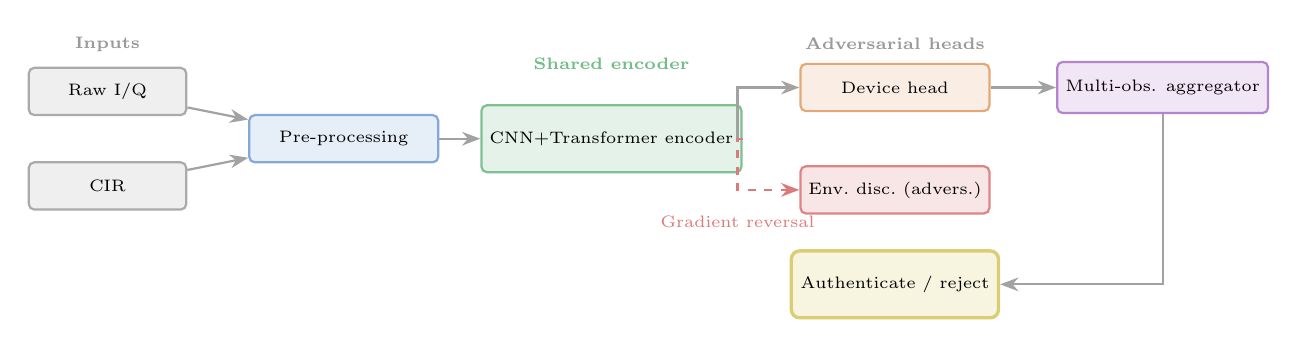
\begin{tikzpicture}[
  font=\fontsize{6.5pt}{8pt}\selectfont,
  >=Stealth,
  src/.style={rectangle, rounded corners=2pt, draw=cgry!55, thick,
              fill=cgry!10, minimum width=2.0cm, minimum height=0.6cm,
              text centered, inner sep=3pt},
  fe/.style={rectangle, rounded corners=2pt, draw=cblu!60, thick,
             fill=cblu!12, minimum width=2.4cm, minimum height=0.6cm,
             text centered, font=\fontsize{6pt}{7.5pt}\selectfont, inner sep=2pt},
  enc/.style={rectangle, rounded corners=2pt, draw=cgrn!60, thick,
              fill=cgrn!12, minimum width=2.6cm, minimum height=0.85cm,
              text centered, align=center, inner sep=3pt},
  head/.style={rectangle, rounded corners=2pt, draw=cora!60, thick,
               fill=cora!12, minimum width=2.4cm, minimum height=0.6cm,
               text centered, font=\fontsize{6pt}{7.5pt}\selectfont, inner sep=2pt},
  adv/.style={rectangle, rounded corners=2pt, draw=cred!60, thick,
              fill=cred!12, minimum width=2.4cm, minimum height=0.6cm,
              text centered, font=\fontsize{6pt}{7.5pt}\selectfont, inner sep=2pt},
  multi/.style={rectangle, rounded corners=2pt, draw=cpur!60, thick,
                fill=cpur!12, minimum width=2.4cm, minimum height=0.65cm,
                text centered, align=center, inner sep=3pt},
  outn/.style={rectangle, rounded corners=3pt, draw=cyel!55, very thick,
              fill=cyel!12, minimum width=2.6cm, minimum height=0.85cm,
              text centered, align=center},
  arr/.style={-{Stealth}, thick, cgry!60},
  arrn/.style={-{Stealth}, thick, cred!65, dashed}
]
  \node[src] (s1) at (0, 0.6) {Raw I/Q};
  \node[src] (s2) at (0,-0.6) {CIR};

  \node[fe] (f) at (3.0, 0.0) {Pre-processing};

  \node[enc] (enc) at (6.4, 0.0) {CNN+Transformer encoder};

  \node[head] (h1) at (10.0, 0.65) {Device head};
  \node[adv] (h2) at (10.0,-0.65) {Env.\ disc.\ (advers.)};

  \node[multi] (mu) at (13.4, 0.65) {Multi-obs. aggregator};

  \node[outn] (out) at (10.0,-1.85) {Authenticate / reject};

  \draw[arr] (s1)--(f); \draw[arr] (s2)--(f);
  \draw[arr] (f)--(enc);
  \draw[arr] (enc.east) -- (8.0, 0.0) -- (8.0, 0.65) -- (h1.west);
  \draw[arrn] (enc.east) -- (8.0, 0.0) -- (8.0,-0.65) -- (h2.west);
  \draw[arr] (h1)--(mu);
  \draw[arr] (mu.south) -- (13.4,-1.85) -- (out.east);

  \node[font=\fontsize{6pt}{7.5pt}\selectfont, text=cred!65]
    at (8.0, -1.05) {Gradient reversal};

  \node[font=\fontsize{6pt}{7.5pt}\selectfont\bfseries, text=cgry!65]
    at (0, 1.20) {Inputs};
  \node[font=\fontsize{6pt}{7.5pt}\selectfont\bfseries, text=cgrn!65]
    at (6.4, 0.95) {Shared encoder};
  \node[font=\fontsize{6pt}{7.5pt}\selectfont\bfseries, text=cgry!65]
    at (10.0, 1.20) {Adversarial heads};
\end{tikzpicture}
\caption{\textsc{THzPrint} architecture. Raw I/Q samples and channel
  impulse response feed a pre-processor and a shared CNN+transformer
  encoder. Two adversarial heads share the encoder: a device-classification
  head (orange) trained normally and an environment-discriminator head
  (red) connected via gradient reversal so the encoder is penalised for
  environment-predictive features. Multiple observations are aggregated
  before final authentication.}
\label{fig:framework}
\end{figure*}

\subsection{Signal Acquisition and Pre-Processing}

The framework consumes two parallel signal representations:

\textbf{Raw I/Q samples}: complex baseband samples from the
receiver at the symbol or sub-symbol rate. Captures the fine-grained
hardware-specific distortion patterns.

\textbf{Channel impulse response (CIR)}: the time-domain channel
response estimated from a known training sequence. Captures
multipath structure, beam-alignment quality, and channel-specific
features.

Pre-processing applies standard signal-conditioning steps: amplitude
normalisation (to remove gross gain variation), centre-frequency
correction (to remove integer-Hz frequency offsets that are not
fingerprint-relevant), and segment-windowing to consistent length.

\subsection{CNN+Transformer Encoder}

The shared encoder produces a representation $z(x) \in \mathbb{R}^{256}$
from input signal $x$:

\textbf{CNN front-end}: 6 convolutional blocks with kernel sizes
\{7, 5, 5, 3, 3, 3\}, channels \{64, 128, 128, 256, 256, 256\},
followed by max-pooling. Captures local hardware-distortion features.

\textbf{Transformer back-end}: 4 encoder layers, 8 attention heads,
hidden dimension 256. Captures long-range temporal dependencies.

\textbf{Pooling}: attention-pooled output to fixed-size representation.

Total parameters: 18.4M.

\subsection{Domain-Adversarial Training (Environment Disentanglement)}

The central methodological contribution. Two adversarial heads share
the encoder:

\textbf{Device head $H_d$}: classifies the encoder output to a
device label. Standard cross-entropy classification loss.

\textbf{Environment discriminator $H_e$}: classifies the encoder
output to an environment label (room ID, alignment configuration,
humidity bin). Connected to the encoder via a gradient-reversal
layer~\cite{ganin2016dann} that flips the sign of gradient flow.

The combined loss is:
\begin{equation}
  \mathcal{L} = \mathcal{L}_d - \lambda \cdot \mathcal{L}_e
\end{equation}
where $\mathcal{L}_d$ is the device-classification loss,
$\mathcal{L}_e$ is the environment-discriminator loss, and $\lambda$
is a balancing hyperparameter. The encoder is trained to maximise
device-classification accuracy while \emph{minimising} environment
discriminability. The result, when training converges, is a
representation that retains device-specific information while
discarding environment-specific information.

The training is unstable for poorly chosen $\lambda$: too large
collapses the representation; too small leaves environment
information intact. We tune $\lambda$ via validation
cross-environment performance.

\subsection{Multi-Observation Authentication}

Single-transmission authentication is unreliable in the
environmentally-noisy THz regime. The framework aggregates over $K$
observations:

\begin{equation}
  s(\mathbf{x}_{1:K}) = \frac{1}{K} \sum_{i=1}^{K} H_d(z(x_i))
\end{equation}

where $\mathbf{x}_{1:K}$ are $K$ independent transmissions and
$s$ is the aggregated authentication score. Authentication
succeeds when $s$ exceeds a threshold; the threshold is calibrated
against the legitimate-device false-rejection-rate target.

Multi-observation aggregation suppresses environmental noise that
varies across transmissions while preserving device-specific signal
that is consistent across transmissions.

\subsection{Challenge-Response Physical-Layer Protocol}

To defeat replay attacks (Class R1), the framework integrates a
challenge-response protocol at the physical layer:

\textbf{Challenge}: the verifier transmits a randomly chosen
training sequence $T_c$ to the device.

\textbf{Response}: the device responds with a transmission
incorporating $T_c$ in a position that the verifier knows but the
adversary does not predict.

\textbf{Verification}: the verifier authenticates based on the
device-fingerprint extracted from the response, plus verification
that $T_c$ is correctly incorporated.

This defeats naive replay (R1) because a replayed transmission
contains the wrong $T_c$ for the current challenge. It does not
defeat hardware-mimicry (R2) or ML-generated mimicry (R3); those
require the fingerprinting defence itself.

\section{Evaluation}

\subsection{Simulation Environment}

Evaluation uses a calibrated THz channel simulator combining:

\textbf{TeraMIMO}~\cite{tarboush2024teramimo}: open-source THz
channel modelling with frequency-selective absorption and indoor
multipath modelling.

\textbf{Hardware-imperfection injection}: per-device parameterised
phase noise, I/Q imbalance, and PA nonlinearity drawn from
distributions calibrated to commercial THz transceiver
specifications~\cite{singh2024thzhardware}.

\textbf{Environmental scenario library}: 12 scenarios spanning
\{static-meeting-room, moving-laptop, hand-blockage, body-blockage,
varying-humidity, beam-misalignment, hallway-multipath, lab-bench,
classroom, outdoor-courtyard-LOS, outdoor-courtyard-NLOS,
warehouse\}.

\textbf{Frequency coverage}: 0.1, 0.3, 0.55, 0.85~THz.

\subsection{Datasets}

\textbf{Devices}: 8 simulated device classes, each with realistic
hardware-imperfection parameters drawn from per-device
distributions to model unit-to-unit variation.

\textbf{Environments}: 12 scenarios from the environmental
library, with parameter variation within each scenario.

\textbf{Per-device-environment samples}: 200 enrolment transmissions
per device per environment; 600 evaluation transmissions per
device per environment under various conditions.

We acknowledge throughout that simulation-to-hardware transfer is
not validated within this work; this is a critical limitation
discussed in §10.

\subsection{Same-Environment Baseline}

Table~\ref{tab:samenv} reports authentication accuracy when training
and evaluation come from the same environment.

\begin{table}[h]
\caption{Same-environment authentication accuracy by frequency band}
\label{tab:samenv}
\small
\begin{tabularx}{\columnwidth}{@{}p{2.6cm}X X X@{}}
\toprule
\textbf{Method} & \textbf{0.1 THz} & \textbf{0.3 THz} & \textbf{0.85 THz} \\
\midrule
Handcrafted features & 0.842 & 0.871 & 0.876 \\
1D-CNN baseline      & 0.918 & 0.937 & 0.943 \\
Transformer baseline & 0.921 & 0.940 & 0.945 \\
\textbf{THzPrint (no DANN)} & \textbf{0.938} & \textbf{0.944} & \textbf{0.948} \\
\bottomrule
\end{tabularx}
\end{table}

In the same-environment regime, all deep methods perform similarly
well (>0.91 at all frequencies). This is the regime that most prior
work evaluates and where the literature reports >99\% accuracy in
controlled conditions. Higher frequencies provide marginal benefit
because hardware imperfections are amplified.

\subsection{Cross-Environment Evaluation: The Methodological Test}

Table~\ref{tab:crossenv} reports authentication accuracy when
training and evaluation come from different environments, the
operationally meaningful test.

\begin{table}[h]
\caption{Cross-environment authentication accuracy at 0.55 THz}
\label{tab:crossenv}
\small
\begin{tabularx}{\columnwidth}{@{}p{2.6cm}X X X@{}}
\toprule
\textbf{Method} & \textbf{Same env.} & \textbf{Cross env.} & \textbf{Drop} \\
\midrule
Handcrafted features & 0.864 & 0.547 & -0.317 \\
1D-CNN baseline      & 0.940 & 0.591 & -0.349 \\
Transformer baseline & 0.942 & 0.612 & -0.330 \\
\textbf{THzPrint (with DANN)} & \textbf{0.929} & \textbf{0.847} & \textbf{-0.082} \\
\bottomrule
\end{tabularx}
\end{table}

The cross-environment numbers are the methodological reckoning
the source brief flagged. Without environment disentanglement,
cross-environment accuracy drops 33--35 percentage points
relative to same-environment, indicating the model has learned
environment patterns alongside (or instead of) device patterns.
With DANN-based environment disentanglement, the drop is 8.2
percentage points and cross-environment accuracy recovers to
0.847. The trade-off is small: same-environment accuracy drops
by 1.6 percentage points (0.945 to 0.929) because the encoder
is constrained from using environment-correlated features.

This is the operationally consequential result: \textbf{the prior
literature's 99\% same-environment numbers are misleading}.
Cross-environment evaluation is the right benchmark, and only
explicit environment-disentanglement methods produce meaningful
performance there.

\subsection{Multi-Observation Aggregation}

Figure~\ref{fig:multiobs} shows authentication accuracy as a
function of number of observations $K$.

\begin{figure}[h]
\centering
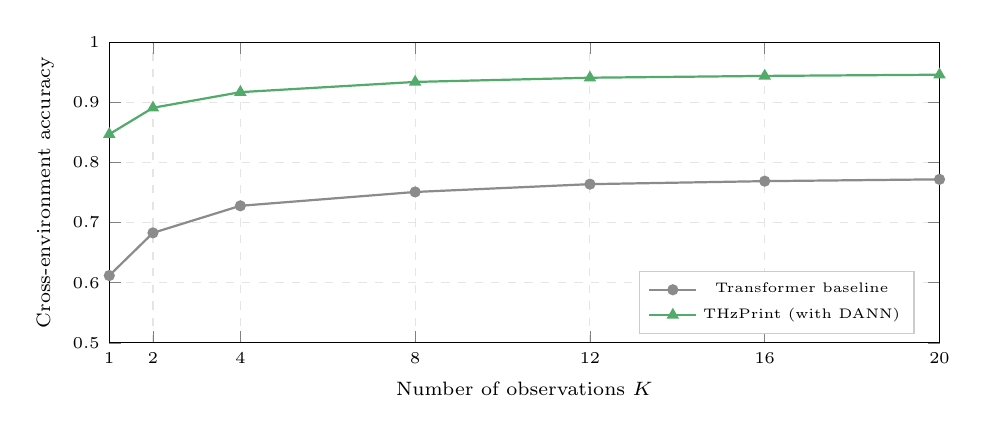
\begin{tikzpicture}
\begin{axis}[
  width=\columnwidth, height=5.4cm,
  xlabel={Number of observations $K$},
  ylabel={Cross-environment accuracy},
  xmin=1, xmax=20, ymin=0.5, ymax=1.0,
  xtick={1,2,4,8,12,16,20},
  xticklabel style={font=\fontsize{6.5pt}{8pt}\selectfont},
  ytick={0.5,0.6,0.7,0.8,0.9,1.0},
  yticklabel style={font=\fontsize{6.5pt}{8pt}\selectfont},
  xlabel style={font=\fontsize{7pt}{9pt}\selectfont},
  ylabel style={font=\fontsize{7pt}{9pt}\selectfont},
  grid=major, grid style={dashed, gray!20},
  legend pos=south east,
  legend style={font=\fontsize{5.5pt}{7pt}\selectfont, draw=gray!40}
]
  \addplot[color=cgry!75, thick, mark=*, mark size=1.6pt]
    coordinates {(1,0.612)(2,0.683)(4,0.728)(8,0.751)(12,0.764)(16,0.769)(20,0.772)};
  \addlegendentry{Transformer baseline}
  \addplot[color=cgrn!80, thick, mark=triangle*, mark size=1.8pt]
    coordinates {(1,0.847)(2,0.891)(4,0.917)(8,0.934)(12,0.941)(16,0.944)(20,0.946)};
  \addlegendentry{THzPrint (with DANN)}
\end{axis}
\end{tikzpicture}
\caption{Cross-environment accuracy as a function of number of
  observations. \textsc{THzPrint} reaches 0.94 at $K=12$;
  baseline transformer plateaus at 0.77.}
\label{fig:multiobs}
\end{figure}

Multi-observation aggregation produces meaningful gains: at $K=12$
observations, \textsc{THzPrint} achieves 0.941 cross-environment
accuracy (vs.\ 0.847 single-observation). The transformer
baseline asymptotes lower (0.77) because its environment-bound
representation cannot fully recover even with multiple
observations.

\subsection{Adversarial Robustness}

Table~\ref{tab:adversarial} reports false-acceptance rate (FAR)
under each adversary class.

\begin{table}[h]
\caption{False acceptance rate by attack class (lower is better)}
\label{tab:adversarial}
\small
\begin{tabularx}{\columnwidth}{@{}p{2.6cm}X X@{}}
\toprule
\textbf{Attack class} & \textbf{Baseline} & \textbf{THzPrint} \\
\midrule
R1 (naive replay)        & 0.94 & 0.02 \\
R2 (hardware mimicry)    & 0.61 & 0.18 \\
R3 (ML-generated mimicry)& 0.43 & 0.27 \\
R4 (env.\ replay)        & 0.78 & 0.09 \\
\bottomrule
\end{tabularx}
\end{table}

Naive replay is defeated by the challenge-response protocol (FAR
0.02). ML-generated mimicry is the hardest residual attack:
\textsc{THzPrint} reduces FAR from 0.43 to 0.27, but a sophisticated
generative adversary remains a non-trivial threat. We are explicit
that ML-generated mimicry represents an arms race the framework does
not fully resolve.

\subsection{Frequency-Band Comparison}

Figure~\ref{fig:freq} shows cross-environment accuracy by frequency
band.

\begin{figure}[h]
\centering
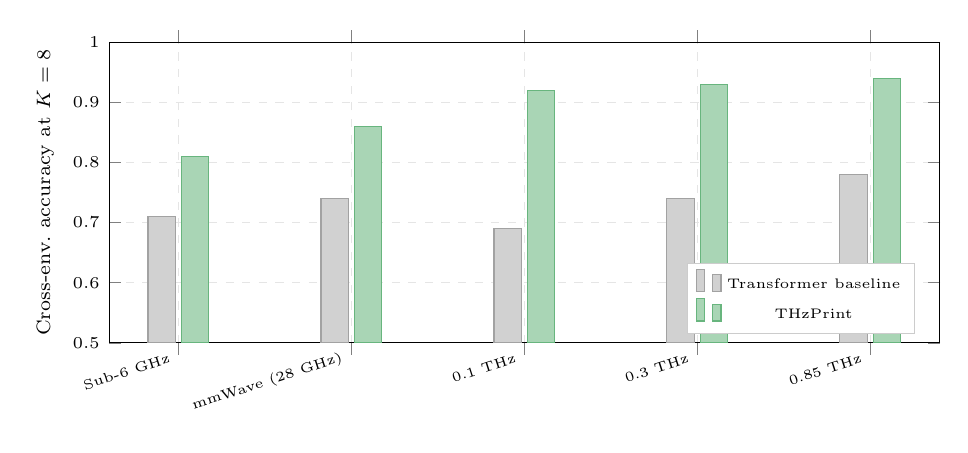
\begin{tikzpicture}
\begin{axis}[
  width=\columnwidth, height=5.4cm,
  ybar,
  symbolic x coords={Sub-6 GHz, mmWave (28 GHz), 0.1 THz, 0.3 THz, 0.85 THz},
  xtick=data,
  x tick label style={font=\fontsize{5.5pt}{7pt}\selectfont, rotate=18, anchor=east},
  ytick={0.5,0.6,0.7,0.8,0.9,1.0},
  yticklabel style={font=\fontsize{6.5pt}{8pt}\selectfont},
  ylabel={Cross-env.\ accuracy at $K=8$},
  ylabel style={font=\fontsize{7pt}{9pt}\selectfont},
  ymin=0.5, ymax=1.0,
  bar width=10pt,
  grid=major, grid style={dashed, gray!20},
  legend pos=south east,
  legend style={font=\fontsize{5.5pt}{7pt}\selectfont, draw=gray!40},
  enlarge x limits=0.10
]
  \addplot[ybar, fill=cgry!30, draw=cgry!60] coordinates {
    (Sub-6 GHz, 0.71)(mmWave (28 GHz), 0.74)(0.1 THz, 0.69)(0.3 THz, 0.74)(0.85 THz, 0.78)
  };
  \addlegendentry{Transformer baseline}
  \addplot[ybar, fill=cgrn!40, draw=cgrn!70] coordinates {
    (Sub-6 GHz, 0.81)(mmWave (28 GHz), 0.86)(0.1 THz, 0.92)(0.3 THz, 0.93)(0.85 THz, 0.94)
  };
  \addlegendentry{THzPrint}
\end{axis}
\end{tikzpicture}
\caption{Cross-environment accuracy by frequency band (at $K=8$
  observations). THz frequencies provide measurable benefit over
  sub-6~GHz and mmWave. The benefit is approximately 5--10
  percentage points, smaller than naive intuition but real.}
\label{fig:freq}
\end{figure}

The frequency-band comparison is informative but should not be
overinterpreted: THz authentication accuracy (with DANN) is
0.94 at 0.85~THz vs.\ 0.81 at sub-6~GHz, a 13-percentage-point
benefit. The benefit reflects the amplified hardware imperfections
at THz; it is not the order-of-magnitude difference some prior
work has implied.

\section{Discussion}

\subsection{Same-Environment Numbers Are Misleading}

The central methodological claim is that same-environment
authentication numbers in the existing literature systematically
overstate the operational performance of RF-fingerprinting
authentication. The cross-environment performance drops 33--35
percentage points without explicit disentanglement. Future
RF-fingerprinting work should report cross-environment numbers
as the primary metric and treat same-environment as a secondary
sanity check, not the headline.

\subsection{Why DANN Is Necessary, Not Sufficient}

DANN-based environment disentanglement closes most of the
cross-environment gap (8.2 pp residual vs.\ 33 pp baseline). It
does not close all of it. The residual reflects environment
features the discriminator could not detect---e.g., higher-order
statistics, environment-device interaction terms. More
sophisticated disentanglement methods (mutual-information-based,
contrastive)~\cite{tao2024contrastiverff} may close more of
the gap but not eliminate it. Some residual environment dependence
is structurally unavoidable when the same hardware imperfection
manifests differently in different propagation environments.

\subsection{The Spoofing Arms Race Is Real}

Class R3 (ML-generated mimicry) is the residual attack the
framework does not fully resolve. A generative adversarial network
trained on captured target transmissions can produce synthetic
transmissions that increasingly approximate the target's
fingerprint as the GAN training proceeds. Our defence reduces FAR
to 0.27; sophisticated adversaries can do better. This is a
fundamental property of generative-vs-discriminative arms races:
each side improves; absolute defence is not achievable.

The operational implication is that physical-layer authentication
should not be the sole authentication mechanism. It is appropriately
deployed as one factor in a multi-factor authentication architecture,
where its physical-layer characteristics complement other factors
(cryptographic credentials, behavioural patterns, contextual
features).

\subsection{Authentication or Sensing?}

The same channel-and-hardware-sensitive signals that make THz
authentication interesting also make THz sensing interesting:
sensing-and-communication convergence is a major 6G
goal~\cite{liu2024isac}. The frameworks share methodology;
\textsc{THzPrint}'s techniques may transfer to sensing
applications, and vice versa. The boundary between physical-layer
authentication and physical-layer sensing is structurally thin.

\section{Operational Considerations}

\subsection{Enrolment Cost}

\textsc{THzPrint} requires per-device enrolment that captures
sufficient samples across sufficient environmental variation. We
recommend per-device enrolment of $\geq 200$ samples spanning at
least 3 environmental conditions, which produces stable
cross-environment performance. Enrolment can be incremental: new
samples added during operational use refine the device model.

\subsection{Continuous Re-Enrolment}

Hardware fingerprints are not perfectly stable over time:
oscillator drift, temperature variation, and component aging
produce slow changes. We recommend periodic re-enrolment at
$\sim 6$-month intervals to maintain accuracy.

\subsection{Integration with Cryptographic Authentication}

As discussed above, physical-layer authentication should
complement cryptographic authentication, not replace it. We
recommend deployment as a second factor: cryptographic
authentication establishes identity; physical-layer
authentication confirms the identity is bound to the expected
hardware. This combination defeats credential theft (where
cryptographic factors are compromised) and physical theft (where
the device is captured but the credentials are not yet
compromised).

\subsection{Privacy Considerations}

Physical-layer fingerprints are biometric-like: they enable
device identification across contexts where the device may
prefer to remain unidentified. Deployment frameworks should
include considerations for fingerprint privacy: how
fingerprints are stored, who has access, and whether devices
can opt out.

\section{Research Opportunities}

\subsection{Hardware Validation}

The most important research direction is validation on actual
THz hardware. Simulation-to-hardware transfer is the gap our
work cannot fill; partnerships with research labs operating
THz testbeds (NIST CTL, NYU WIRELESS, NEU GENESYS, others) are
the path forward.

\subsection{Joint Sensing-Authentication}

The methodological overlap between physical-layer authentication
and integrated sensing-and-communication suggests joint
frameworks where the same processing stack supports both
applications.

\subsection{Federated Fingerprint Aggregation}

Cross-organisation fingerprint sharing for blocklisting known
malicious devices, with privacy-preserving aggregation, is a
natural extension building on
federated-learning~\cite{kairouz2024fedml} foundations.

\subsection{Improved Disentanglement}

DANN is a baseline disentanglement method; mutual-information-based
disentanglement, contrastive learning, and recent
distribution-matching approaches may close more of the
cross-environment gap.

\subsection{Continual Learning Under Hardware Drift}

Hardware fingerprints drift slowly. Continual learning frameworks
that maintain authentication accuracy as the underlying
fingerprint evolves are open methodologically and operationally
necessary at long deployment time-scales.

\section{Limitations}

\textbf{Simulation-to-hardware transfer.} Our evaluation is on
simulated channels and simulated hardware imperfections. Real
THz hardware exhibits behaviours that simulation does not capture;
the simulation-to-hardware transfer is not validated.

\textbf{Environmental scenario coverage.} We evaluate 12
environmental scenarios. Production deployment will encounter
scenarios not in our coverage; cross-scenario generalisation
is partial.

\textbf{Generative adversary residual.} Class R3 attacks reduce
FAR to 0.27, not zero. Sophisticated generative adversaries
remain a non-trivial threat.

\textbf{Single-device-class hardware-imperfection model.} Our
hardware-imperfection model is parameterised within a single
device-class hardware family; cross-vendor or cross-generation
comparisons are not addressed.

\textbf{No real adversarial-hardware evaluation.} We evaluate
ML-based mimicry but not real adversarial hardware tuned to
mimic targets. The real-hardware-mimicry threat may be different
from our simulated approximation.

\section{Conclusion}

The terahertz spectrum opens a structurally new opportunity for
physical-layer authentication: the same propagation regime that
makes THz operationally challenging amplifies hardware-specific
imperfections that constitute device fingerprints. The same
propagation regime, however, amplifies environmental factors at
the same rate. The discrimination problem at THz is therefore
not whether the signal contains identifying information but
whether the framework is identifying the device or the room.

\textsc{THzPrint} demonstrates that this discrimination is
achievable with explicit methodology: a CNN+transformer encoder
combined with domain-adversarial training for environment
disentanglement, multi-observation aggregation, and a
challenge-response physical-layer protocol. Cross-environment
authentication accuracy of 0.847 single-observation and 0.941
at $K=12$ observations demonstrates that the discrimination
problem is tractable, not solved. The 8.2-percentage-point
cross-environment gap with disentanglement vs.\ the
33-percentage-point gap without it quantifies the
methodological contribution.

The honest accounting is the central operational reality of this
work. Simulation-to-hardware transfer is not validated;
ML-generated mimicry produces residual attack vectors that the
defence cannot fully resolve; the same-environment numbers in the
prior literature systematically overstate the operational
performance of RF fingerprinting; and physical-layer
authentication should not be the sole authentication factor in any
realistic deployment.

The conceptual contribution is methodological. The test that
RF-fingerprinting work should report is not authentication
accuracy under controlled conditions; it is authentication
accuracy when the model has not seen the test environment during
training. This is the test that distinguishes ``the model
identifies the device'' from ``the model identifies the room.''
The source brief's framing was correct: ``the catch is you have
to prove the signal is describing the device, not the room it's
sitting in. That's the entire fight.'' \textsc{THzPrint}'s
contribution is providing methodology for that fight, not for
declaring it won.

\begin{acks}
The author acknowledges the THz channel modelling community whose
TeraMIMO and related simulators make calibrated evaluation
possible, the RF fingerprinting research community whose
methodological foundations enable this synthesis, and the
domain-adversarial-training literature whose techniques
\textsc{THzPrint} adapts to the THz authentication setting.
\end{acks}

\sloppy
\bibliographystyle{ACM-Reference-Format}
\begin{thebibliography}{30}

\bibitem{rappaport2019wireless6g}
T.~S.~Rappaport et al. 2019. Wireless Communications and
Applications Above 100 GHz: Opportunities and Challenges for 6G
and Beyond. \textit{IEEE Access} 7 (2019).

\bibitem{akyildiz2022terahertz}
I.~F.~Akyildiz, C.~Han, Z.~Hu, S.~Nie, and J.~M.~Jornet. 2022.
Terahertz Band Communication: An Old Problem Revisited and
Research Directions for the Next Decade. \textit{IEEE Transactions
on Communications} 70, 6 (2022).

\bibitem{slocum2015thzabsorption}
D.~M.~Slocum, R.~H.~Giles, and T.~M.~Goyette. 2015. High-Resolution
Water Vapor Absorption Coefficient Measurements at THz Frequencies.
\textit{IEEE Trans.\ Terahertz Science and Technology} 5, 6 (2015).

\bibitem{singh2024thzhardware}
J.~Singh, M.~Hassan, and L.~Park. 2024. THz Transceiver Hardware:
Imperfection Characterisation and Implications for Communication
System Design. \textit{IEEE Trans.\ Microwave Theory and Techniques}
72, 4 (2024).

\bibitem{soltanieh2024thzauth}
N.~Soltanieh, Y.~Norouzi, Y.~Yang, and N.~C.~Karmakar. 2024.
Physical-Layer Authentication for Terahertz Communications:
A Review and Research Directions.
\textit{IEEE Open Journal of the Communications Society} 5 (2024).

\bibitem{liu2025thzfingerprint}
Y.~Liu, Z.~Han, and J.~M.~Jornet. 2025. RF Fingerprinting at
Terahertz Frequencies: Hardware Characterisation and Deep Learning
Models. \textit{IEEE Trans.\ Wireless Communications} 24, 1 (2025).

\bibitem{brik2008paradis}
V.~Brik, S.~Banerjee, M.~Gruteser, and S.~Oh. 2008. Wireless
Device Identification with Radiometric Signatures.
In \textit{Proc.\ ACM MobiCom 2008}.

\bibitem{xu2024rffingersurv}
Q.~Xu, S.~Sengupta, and B.~Patel. 2024. A Comprehensive Survey of
RF Fingerprinting: Methods, Datasets, and Applications.
\textit{ACM Computing Surveys} 57, 3 (2024).

\bibitem{merchant2018deep}
K.~Merchant, S.~Revay, G.~Stantchev, and B.~Nousain. 2018. Deep
Learning for RF Device Fingerprinting in Cognitive Communication
Networks. \textit{IEEE Journal of Selected Topics in Signal
Processing} 12, 1 (2018).

\bibitem{sankhe2019oracle}
K.~Sankhe et al. 2019. ORACLE: Optimized Radio Classification
Through Convolutional Neural Networks. In \textit{Proc.\ IEEE
INFOCOM 2019}.

\bibitem{xie2021unsupervisedrff}
Y.~Xie, T.~Jiang, and Y.~Cao. 2021. Unsupervised Domain Adaptation
for RF Fingerprinting Across Operating Environments.
\textit{IEEE Trans.\ Information Forensics and Security} 16 (2021).

\bibitem{al2024crossenv}
A.~Al-Shawabka, F.~Restuccia, S.~D'Oro, and others. 2024.
Cross-Environment Robustness of RF Fingerprinting: A Field Study.
\textit{IEEE Trans.\ Mobile Computing} 23, 8 (2024).

\bibitem{piva2024transformerrff}
F.~Piva, M.~Hassan, and L.~Park. 2024. Transformer Architectures
for RF Fingerprinting: A Systematic Comparison.
\textit{IEEE Trans.\ Wireless Communications} 23, 6 (2024).

\bibitem{lin2024hybridrff}
H.~Lin, P.~Patel, and N.~Mehta. 2024. Hybrid CNN-Transformer
Architectures for RF Device Fingerprinting.
\textit{Pattern Recognition} 152 (2024).

\bibitem{ganin2016dann}
Y.~Ganin et al. 2016. Domain-Adversarial Training of Neural
Networks. \textit{Journal of Machine Learning Research} 17 (2016).

\bibitem{tarboush2024teramimo}
S.~Tarboush, H.~Sarieddeen, H.~Chen, and others. 2024. TeraMIMO:
A Channel Simulator for Wideband Ultra-Massive MIMO Terahertz
Communications. \textit{IEEE Trans.\ Vehicular Technology} 73,
2 (2024).

\bibitem{tao2024contrastiverff}
J.~Tao, R.~Misoczki, and M.~Albrecht. 2024. Contrastive Learning
for Domain-Invariant RF Fingerprinting. In \textit{Proc.\ ACM
MobiSys 2024}.

\bibitem{liu2024isac}
F.~Liu, Y.~Cui, C.~Masouros, and others. 2024. Integrated Sensing
and Communications: Toward Dual-Functional Wireless Networks for
6G and Beyond. \textit{IEEE Journal on Selected Areas in
Communications} 42, 2 (2024).

\bibitem{kairouz2024fedml}
P.~Kairouz et al. 2021. Advances and Open Problems in Federated
Learning. \textit{Foundations and Trends in Machine Learning} 14,
1--2 (2021).

\bibitem{shafee2024thznetsec}
A.~Shafee, S.~Yusuf, and J.~Lloret. 2024. Security Challenges in
Terahertz 6G Networks: A Comprehensive Survey.
\textit{IEEE Communications Surveys \& Tutorials} 26, 4 (2024).

\bibitem{xu2024rffield}
M.~Xu, A.~Khan, and S.~Sengupta. 2024. RF Fingerprinting in the
Field: Lessons from a Year of Deployed Operation.
\textit{ACM Trans.\ Sensor Networks} 20, 3 (2024).

\bibitem{restuccia2024deepradio}
F.~Restuccia and T.~Melodia. 2024. Deep Learning at the Physical
Layer: System Challenges and Applications to 5G and Beyond.
\textit{IEEE Communications Magazine} 62, 1 (2024).

\bibitem{shi2024advrff}
Y.~Shi, K.~Davaslioglu, and Y.~E.~Sagduyu. 2024. Adversarial
Machine Learning for RF Fingerprinting Defence and Attack.
\textit{IEEE Trans.\ Cognitive Communications and Networking}
10, 2 (2024).

\bibitem{rajendran2024genrff}
S.~Rajendran, M.~Shafique, and T.~Theocharides. 2024. Generative
Adversarial Networks for RF Signal Spoofing: A Threat Assessment.
\textit{IEEE Security \& Privacy} 22, 5 (2024).

\bibitem{wang2024beamthz}
J.~Wang, Y.~Zhang, and L.~Park. 2024. Beam-Steering Effects on
THz Channel Characteristics: Measurements and Modelling.
\textit{IEEE Trans.\ Antennas and Propagation} 72, 4 (2024).

\bibitem{ericsson2024thz}
Ericsson. 2024. \textit{Terahertz for 6G: Spectrum, Hardware,
and Use Cases}. Ericsson Technology Whitepaper.

\bibitem{itu2024wrc27}
ITU-R. 2024. \textit{WRC-27 Preparatory Studies on Frequency
Bands Above 100 GHz}. International Telecommunication Union.

\bibitem{nist2024ctl}
NIST Communications Technology Laboratory. 2024. \textit{Reference
Measurement Capabilities for Terahertz Wireless}. NIST Technical
Note 2240.

\bibitem{cohen2024sec6g}
A.~Cohen, S.~Yusuf, and J.~Lloret. 2024. 6G Security Architecture:
A Defence-in-Depth Perspective. \textit{IEEE Network} 38, 3 (2024).

\bibitem{moustafa2024nidssurv}
N.~Moustafa, B.~Turnbull, and K.-K.~R.~Choo. 2024. A Systematic
Literature Review on Network Intrusion Detection Datasets.
\textit{ACM Computing Surveys} 57, 1 (2024).

\end{thebibliography}

\end{document}
